\documentclass[12pt,x11names,a4paper]{article}
\input{preamble}


\newgeometry{margin=2cm}

\pagestyle{fancy}
\fancyhf{}

\rhead{Nørre Gymnasium
}
\cfoot{Side \thepage \hspace{1pt} af \pageref{LastPage}}

%Husk at rette modul og dato!
\lhead{Matematikscreening
}
\chead{30. september 2022
}

\begin{document}

%\includepdf[pages=-]{Forsider/aarsprove_1v.pdf}
\savegeometry{art}

\begin{titlepage}
\newgeometry{margin=0pt}

\begin{minipage}{0.27\textwidth}

\begin{tikzpicture}[overlay]
\fill[top color = NorregGroen!40, bottom color = NorregGroen] (6,10) rectangle (-10,-30);
\end{tikzpicture}
\end{minipage}
\begin{minipage}{0.73\textwidth}
\begin{center}
\phantom{h} \vspace{1cm}\\
\hspace{4cm}
\includegraphics[scale = 1]{Billeder/Norreg.png} \\
\phantom{h} \vspace{5cm}\\
\rule{0.7\textwidth}{0.3mm}\\
\phantom{h}\\
{\fontsize{50}{60}\selectfont Matematik-\\screening}\\
\phantom{h}\\
\rule{0.7\textwidth}{0.3mm}\\
\Large Studentereksamen\\
\Large 2022\\
\Large Version A

\end{center}
\end{minipage}
\end{titlepage}
\loadgeometry{art}

%Udfyld afsnit herunder og lav til egen Latex-fil

%Kopier følgende til overskrift:

%\begin{center}
%\Huge
%Aflevering 1
%\end{center}
%\section*{Opgave 1}
%\stepcounter{section}
\begin{center}
Opgavesætter er delt i to dele:\\
\end{center}
Delprøve 1: 1.0 time kun med den centralt udmeldte formelsamling.\\
Delprøve 2: 2.0 timer med alle hjælpemidler.
\begin{center}
Delprøve 1 består af opgave 1-5.\\
Delprøve 2 består af opgave 6-9.\\
Pointtallet er angivet ud for hvert spørgsmål.\\
Der gives i alt 160 point\\


En del af spørgsmålene er knyttet til mindstekravene.\\
Disse spørgsmål er markeret med grøn farve. 
\end{center}
\section*{Krav til formidling af din besvarelse}

Ved bedømmelse af helhedsindtrykket af besvarelsen af de enkelte opgaver lægges særlig vægt på følgende fire punkter:
\begin{itemize}
\item[$\cdot$] \textbf{Redegørelse og dokumentation for metode} \\
Besvarelsen skal indeholde en redegørelse for den anvendte løsningsstragegi med dokumentation i form af et passende antal mellemregninger \textit{eller} matematiske forklaringer på metoden, når et matematisk værktøjsprogram anvendes.
\item[$\cdot$] \textbf{Figurer, grafer og andre illustrationer} \\
Besvarelsen skal indeholde hensigtsmæssig brug af figurer, grafer og andre illustrationer, og der skal være tydelige henvisninger til brug af disse i den forklarende tekst.
\item[$\cdot$] \textbf{Notation og layout}\\
Besvarelsen skal i overensstemmelse med god matematisk skik opstilles med hensigtsmæssig brug af symbolsprog, og med en redegørelse for den matematiske notation, der indføres og anvendes, og som ikke kan henføres stil standardviden.
\item[$\cdot$] \textbf{Formidling og forklaring}\\
Besvarelsen af rene matematikopgaver skal indeholde en angivelse af givne oplysninger og korte forklaringer knyttet til den anvendte løsningsstrategi beskrevet med brug af almindelig matematisk notation. 

Besvarelsen af opgaver, der omhandler matematiske modeller, skal indeholde en kort præsentation af modellens kontekst, herunder betydning af modellens parametre. De enkelte delspørgsmål skal afsluttes med en præcis konklusion præsenteret i et klart sprog i relation til konteksten.
\end{itemize}

\newpage

\begin{center}
\LARGE
Delprøve uden hjælpemidler (8:30 - 9:30)
\end{center}
\stepcounter{section}

\begin{opgavetekst}{Opgave 1}
En funktion $f$ er givet ved 
\begin{align*}
f(x) = 7x - 21.
\end{align*}
\end{opgavetekst}
\begin{delopgave}{(5 point)}{1}
		Bestem $f(-3)$.
\end{delopgave}
\begin{delopgave}{(5 point)}{2}
	Bestem skæringspunktet mellem grafen for $f$ og førsteaksen.
\end{delopgave}
\begin{opgavetekst}{Opgave 2}
	På Fig. \ref{fig:lines} ses graferne for tre lineære funktioner $f$, $g$ og $h$ med forskrifterne 
	\begin{align*}
		f(x) &= 2x-1,\\
		g(x) &= 4x,\\
		h(x) &= -x+5.
	\end{align*}
	Desuden ses punktet $P(2,y)$, der ligger på skæringen mellem graferne $A$ og $B$.
	\begin{figure}[H]
		\centering
		\begin{tikzpicture}
			\begin{axis}[
				axis lines = center,
				xmin = -3,
				ymin = -1
				]
				\addplot[samples = 10, color = green] {2*x-1};
				\addplot[samples = 10, color = red]	{4*x};
				\addplot[samples = 10, color = blue] {-x+5};
				\node[circle, fill = black, inner sep = 0pt, minimum size = 5pt] at (axis cs: 2,3) {};
				\node at (axis cs:2,4) {$P$};
				\draw[dashed, color = gray, thick] (axis cs: 2,0 ) -- (axis cs:2,3);
				\draw[dashed, color = gray, thick] (axis cs: 0,3 ) -- (axis cs:2,3);
				\node at (axis cs:-0.23,3) {$y$};
				\node[color = blue] at (axis cs:-0.7,7) {$A$};
				\node[color = green] at (axis cs:4,5.5) {$B$};
				\node[color = red] at (axis cs:2,9.5) {$C$};
			\end{axis}
			\node at (9,0.3) {(1)};
			\node at (3.15,7.5) {(2)};
		\end{tikzpicture}
		\caption{Graferne for funktionerne $f$, $g$ og $h$.}
		\label{fig:lines}
	\end{figure}\phantom{h}
\end{opgavetekst}
\begin{delopgave}{\colorbox{NorregGroen!40}{(5 point)}}{1}
	Løs ligningen 
	\begin{align*}
	5x+13 =-2
	\end{align*}
\end{delopgave}

\begin{opgavetekst}{Opgave 3}
To linjer $l$ og $m$ har ligningerne 
\begin{align*}
&l: \ x + y = 0,\\
&m: \ 2x-4y = 6.
\end{align*}
\end{opgavetekst}
\begin{delopgave}{(10 point)}{1}
Find skæringspunktet mellem linjerne $l$ og $m$. 
\end{delopgave}

\begin{opgavetekst}{Opgave 4}

På Fig. \ref{fig:eksp} ses grafen for en aftagende eksponentiel funktion $f$ med forskriften 
\begin{align*}
f(x) = b\cdot a^x.
\end{align*}
\begin{figure}[H]
 \centering
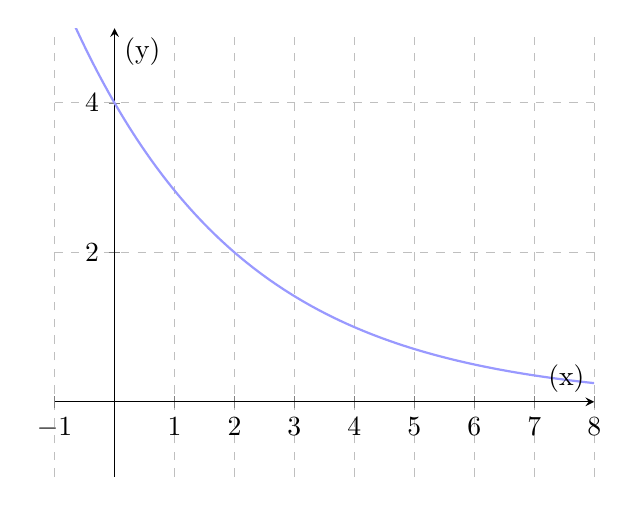
\begin{tikzpicture}
\begin{axis}[grid style = {dashed}, axis lines = middle, xmin = -1, xmax = 8, ymin = -1, ymax = 5, grid,
xtick = {-1,0,1,2,3,4,5,6,7,8}, xlabel = (x), ylabel = (y)
]
\addplot[thick, color = blue!40, samples = 1000, domain = -2:8] {4*0.7071067812^x};

\end{axis}

\end{tikzpicture}
\caption{Graf for eksponentiel funktion $f$.}
\label{fig:eksp}
\end{figure}\phantom{h}
\end{opgavetekst}
\begin{delopgave}{\colorbox{NorregGroen!40}{(5 point)}}{1}
Aflæs koefficienten $b$ på Fig. \ref{fig:eksp}. 
\end{delopgave}
\begin{delopgave}{(5 point)}{2}
Aflæs halveringskonstanten $T_{1/2}$ for $f$ på Fig. \ref{fig:eksp}.
\end{delopgave}

\begin{opgavetekst}{Opgave 5}
Af Fig. \ref{fig:polys} ses parablerne $P_1$, $P_2$ og $P_3$ for tre andengradspolynomier $f$, $g$ og $h$ givet ved henholdsvist
\begin{align*}
f(x) &= x^2 + 2x -3,\\
g(x) &= -x^2 + 2x + 3,\\
h(x) &= x^2-x-2.
\end{align*}
\begin{figure}[H]
\centering
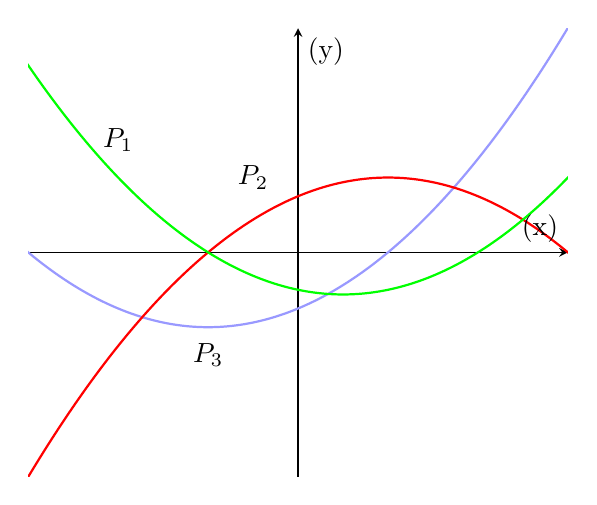
\begin{tikzpicture}
\begin{axis}[axis lines = middle, xmin = -3, xmax = 3, ticks = none, 
xlabel = {(x)},
ylabel = {(y)}
]
\addplot[color = blue!40, thick, samples = 1000] {x^2+2*x-3};
\addplot[color = red, thick, samples = 1000] {-x^2+2*x+3};
\addplot[color = green, thick, samples = 1000] {x^2-x-2};
\node at (axis cs: -2,6) {$P_1$};
\node at (axis cs:-0.5,4) {$P_2$};
\node at (axis cs:-1,-5.5){$P_3$};
\end{axis}
\end{tikzpicture}
\caption{Parablerne $P_1$, $P_2$ og $P_3$ for polynomierne $f$, $g$ og $h$. }
\label{fig:polys}
\end{figure}
\phantom{h}
\end{opgavetekst}

\begin{delopgave}{\colorbox{NorregGroen!40}{(10 point)}}{1}
	Bestem hvilke af parablerne $P_1$, $P_2$ og $P_3$ der hører til polynomierne $f$, $g$ og $h$. 
\end{delopgave}

\begin{delopgave}{(10 point)}{2}
	Bestem rødderne til polynomiet med parablen $P_1$. 
\end{delopgave}

\newpage
\begin{center}
\LARGE
Delprøve med hjælpemidler (8:30-11:30)
\end{center}


\begin{opgavetekst}{Opgave 6}

To funktioner $f$ og $g$ er givet ved 
\begin{align*}
f(x) = \sqrt{7+3x^2}
\end{align*}
og
\begin{align*}
g(x) = x^4-2x+1.
\end{align*}
\end{opgavetekst}

\begin{delopgave}{\colorbox{NorregGroen!40}{(10 point)}}{1}
Tegn graferne for $f$ og $g$ på intervallet $[-1;2]$. 
\end{delopgave}
\begin{delopgave}{(10 point)}{2}
Bestem de to skæringspunkter mellem graferne for $f$ og $g$. 
\end{delopgave}
\begin{delopgave}{(10 point)}{3}
Bestem de sammensatte funktioner $f(g(x))$ og $g(f(x))$. 
\end{delopgave}

\begin{opgavetekst}{Opgave 7}
\begin{center}
\includegraphics[width = 0.7\textwidth]{Billeder/Medicin}
\end{center}
I en person måles til tidspunktet $t = 0$ en koncentration på 157 mg/L af et bestemt lægemiddel. Efter 20 timer er koncentrationen på 112 mg/L. Det antages at koncentrationen i blodet kan beskrives ved en funktion $f$ med forskriften
\begin{align*}
f(x) = b \cdot a^x.
\end{align*}
\end{opgavetekst}

\begin{delopgave}{\colorbox{NorregGroen!40}{(10 point)}}{1}
Bestem tallene $b$ og $a$ for forskriften for $f$.
\end{delopgave}
\begin{delopgave}{\colorbox{NorregGroen!40}{(10 point)}}{2}
Bestem hvad koncentrationen i følge modellen er efter 40 timer. 
\end{delopgave}
\begin{delopgave}{(10 point)}{3}
Bestem halveringskonstanten for $f$ og forklar, hvad dette tal betyder for koncentrationen af lægemiddelet. 
\end{delopgave}

\begin{opgavetekst}{Opgave 8}
\begin{center}
\includegraphics[width = 0.4\textwidth]{Billeder/appelsin}
\end{center}
En grossist af frugt og grønt sælger appelsiner efter følgende prissætning:
\begin{itemize}
\item[$\cdot$] De første 100kg appelsiner koster 20 kr. per kg.
\item[$\cdot$] De næste 900kg appelsiner koster 17 kr. per kg.
\item[$\cdot$] Prisen efter du har købt for 1000kg appelsiner er 15kr. per kg. 
\end{itemize} \phantom{h}
\end{opgavetekst}

\begin{delopgave}{(10 point)}{1}
Indfør passende variable og argumentér for, at prisen for appelsinerne kan beskrives ved funktionen $p$ givet ved
\begin{align*}
p(x) = \begin{cases}
20\cdot x \ &\textnormal{når } x\leq 100,\\
17\cdot x + 300 \ &\textnormal{når }100 < x \leq 1000,\\
15\cdot x + 2300 \ &\textnormal{når } 1000 < x.   
\end{cases}
\end{align*}

\end{delopgave}

\begin{delopgave}{(5 point)}{2}
Bestem prisen for 500kg appelsiner.
\end{delopgave}

\begin{delopgave}{(10 point)}{3}
Hvor mange kg appelsiner kan man købe for 20.000 kr?
\end{delopgave}


\begin{opgavetekst}{Opgave 9}
En uspecificeret person har lavet målingerne, der ses af Tab. \ref{tab:tabel}. 
\begin{table}[H]
\centering
\begin{tabular}{c|c|c|c|c|c|c|c|c|c|c}
$x$ & 0 & 1 & 2 & 3 & 4 & 5 & 6 & 7 & 8 & 9\\
\hline 
$y$ & 11.6 & 4.3 & 2.6 & 0.9 & 1.7 & 0.1 & 0.0 & -0.1 &-0.9& 1.4
\end{tabular}
\caption{Uspecificeret data fra uspecificeret person}
\label{tab:tabel}
\end{table}
Personen har glemt, hvad det er han/hun har målt på, så vedkommende har ingen idé om, hvordan sammenhængen mellem $x$ og $y$ bør være.
\end{opgavetekst}

\begin{delopgave}{\colorbox{NorregGroen!40}{(10 point)}}{1}
Lav lineær regression og eksponentiel regression på datasættet fra Tab. \ref{tab:tabel}.
\end{delopgave}
\begin{delopgave}{(10 point)}{2}
Lav regressionsanalyse på de to regressionsmodeller og afgør ved hjælp af residualerne til modellerne, hvilken af modellerne, der beskriver datasættet bedst. 
\end{delopgave}

\end{document}



